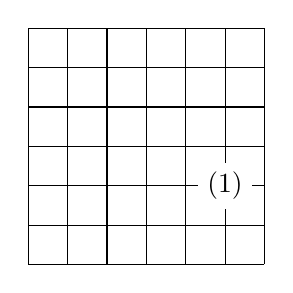
\begin{tikzpicture}[scale=.5]
    \begin{scope}
        \draw (0 ,0) grid (6, 6);

        \fillstone{1}{2}{matblack}
        \fillstone{1}{3}{matblack}
        \fillstone{2}{4}{matblack}
        \fillstone{3}{3}{matblack}
        \fillstone{4}{3}{matblack}
        \node[fill=white, anchor=center] at (5,2) {(1)};
        \fillstone{4}{1}{matblack}
        \fillstone{3}{1}{matblack}
        \fillstone{2}{1}{matblack}

        \fillstone{2}{2}{matgray}
        \fillstone{2}{3}{matgray}
        \fillstone{3}{2}{matgray}
        \fillstone{4}{2}{matgray}
        \fillstone{3}{4}{matgray}
        \fillstone{4}{4}{matgray}
    \end{scope}
\end{tikzpicture}
